% Fakesection 序言之前

\RequirePackage[l2tabu, orthodox]{nag}
\RequirePackage{ifxetex}
\RequireXeTeX

\documentclass{article}

%颜色
\usepackage{xcolor}

%长度
\usepackage{printlen}
\uselengthunit{mm}

%图形
\usepackage{pifont}
\usepackage{ean13isbn}
\usepackage{qrcode}
\usepackage{pdfpages}
\usepackage{overpic}
\usepackage{graphicx}
\graphicspath{{./src/}}
\usepackage{media9}
\usepackage{wallpaper}
\usepackage{wrapfig}

%表格
\usepackage{tabu}
\usepackage{longtable}
\usepackage{booktabs}
\usepackage{diagbox}
\usepackage{multicol}
\usepackage{multirow}
\usepackage{makecell}
\usepackage{fancybox}
\usepackage{colortbl}
\usepackage{tcolorbox}
\tcbuselibrary{skins}
\tcbuselibrary{breakable}
\tcbuselibrary{theorems}
\tcbuselibrary{listings}
\tcbuselibrary{xparse}
\tcbuselibrary{minted}% 用minted排版代码
\usepackage{fvextra}
\usepackage{csvsimple}
\usepackage{boxedminipage2e}

%公式
\usepackage{amsmath}
\usepackage{amsthm}
\usepackage{amsfonts}
\usepackage{amssymb}
\usepackage{amsbsy}
\usepackage{amsopn}
\usepackage{amstext}
\usepackage{mathrsfs}
\usepackage{bm}
\usepackage{textcomp}
\usepackage{latexsym}
\usepackage{exscale}
\usepackage{relsize}
%\usepackage{xymtex}
\usepackage{physics}
\usepackage{siunitx}
\usepackage{hologo}
\usepackage{cases}

%文字
\usepackage{csquotes}
\usepackage{microtype}
\usepackage[heading=true]{ctex}
\setCJKfamilyfont{zhsong}[AutoFakeBold = {2.17}]{SimSun}
\renewcommand*{\songti}{\CJKfamily{zhsong}}

%正文
\usepackage{fancyhdr}
\usepackage{geometry}
\usepackage{lastpage}
\usepackage{indentfirst}
\usepackage{setspace}
\renewcommand\arraystretch{1}

%非正文
\usepackage{makeidx}
\makeindex
\usepackage{epigraph}
\usepackage{varwidth}
\usepackage{exercise}
\usepackage{tasks}

%参考文献
\usepackage{morewrites}
\renewcommand{\thefootnote}{\fnsymbol{footnote}}
\usepackage[resetlabels]{multibib}

%标题
\usepackage{caption}
\usepackage{subcaption}
\DeclareCaptionLabelFormat{andtable}%
{#1#2~\&~\tablename\thetable}
\newcounter{sub}

%其它
\usepackage{atbegshi}
\usepackage{lipsum}

\csname
endofdump
\endcsname

%代码
\usepackage{minted}

%链接%与beamer 冲突
\usepackage
[	colorlinks = true,
linkcolor = gray,
citecolor = gray,
backref=page
]{hyperref}

%枚举%与beamer 干涉
\usepackage{enumitem}
\setlist[enumerate, 2]
{	fullwidth,
	label = \alph*.,
	font = \textup,
	itemindent=2em
}

%标题%与beamer 冲突
\usepackage{titlesec}
%\titleformat{\chapter}{\centering\Huge\bfseries}{实验\chinese{chapter}~}{0pt}{}
\titleformat{\section}{\centering\LARGE\bfseries}{\S\ifthenelse{\value{section}=0}{}{\thesection}~}{0pt}{}
%\titleformat{\subsection}{\Large}{\chinese{subsection}、~}{0pt}{}
%\titleformat{\subsubsection}{\large}{\arabic{subsubsection}.~}{0pt}{}

\begin{document}

\section{研究内容及研究方法}%
\label{sec:研究内容及研究方法}

\subsection{研究内容}%
\label{sub:研究内容}

进入二十一世纪后,军事和民事领域对于红外成像的技术提出了更高的要求,由于红外焦平面探测器具有高空间分辨力,探测能力强,帧频高等优点,其成为了红外成像技术的主流器件。但由于目前探测器的加工工艺,材料,温度影响等原因,导致每个探测元间对相同红外光子流的响应并不一致,存在着固有图形噪声,称为红外焦平面阵列的非均匀性。而非均匀性校正技术是红外图像处理中的一项关键技术,直接影响到最后输出图像的质量。此次科研训练便对此技术进行了一定的研究,在查阅相关的文档后,最终在BP神经网络算法上进行了一定修改,并取得了一定校正结果。

\subsection{研究方法}%
\label{sub:研究方法}

\subsubsection{BP神经网络算法}%
\label{ssub:BP神经网络算法}

如图\ref{fig:神经网络},BP (back propagation)神经网络是1986年由Rumelhart和McClelland为首的科学家提出的概念,是一种按照误差逆向传播算法训练的多层前馈神经网络,是目前应用最广泛的神经网络。

\begin{figure}[htpb]
	\centering
	\includegraphics[width=0.4\linewidth]{BP.pdf}
	\caption{神经网络}
	\label{fig:神经网络}
\end{figure}

人工神经网络无需事先确定输入输出之间映射关系的数学方程,仅通过自身的训练,学习某种规则,在给定输入值时得到最接近期望输出值的结果。作为一种智能信息处理系统,人工神经网络实现其功能的核心是算法。BP神经网络是一种按误差反向传播 (简称误差反传)训练的多层前馈网络,其算法称为BP算法,它的基本思想是梯度下降法,利用梯度搜索技术,以期使网络的实际输出值和期望输出值的误差均方差为最小。

\subsubsection{针对BP神经算法的进一步改进}%
\label{ssub:针对BP神经算法的进一步改进}

在红外加平面的非均匀性校正算法中,BP神经网络算法一般要求目标场景与红外焦平面阵列IRFPA器件相对运动以使得IRFPA器件中所有的探测单元在一段时间内所接收到的目标场景辐射满足一定的统计假设。但是由于场景的多样性,一些假设不一定会得到满足,因此BP神经网络算法伴随着一定的鬼影问题。尤其当IRFPA由静止状态突然转向运动时,会出现鬼影。而IRFPA由静止状态转为运动,是由于出现一定的高频分量。高频分量决定了图像的细节,如图\ref{fig:像素模板为4个像素},传统的BP神经网络算法中对于像元的估计值$ T(i,j)= \dfrac{Y(i,j+1)+Y(i,j-1)+Y(i-1,j)+Y(i+1,j)}{4} $,其本身属于一个低通的模板操作,在一定的程度上限制了高频分量的通过。因而只需要对像元的估计值算式进行修改便可以对其进行改进。

在数字图像处理中,中值滤波和百分比滤波两种非线性滤波方式,都可以做到对于图像高频分量的保护和平滑的作用。

为了方便器件,考虑中值滤波方式,由于中值滤波最好的效果一般在9到13个像素之间,又考虑到红外焦平面像元之间的对称性,所以最后模板操作为9和13个像素两种模板,如图\ref{fig:像素模板为9个像素}和\ref{fig:像素模板为13个像素}。

\begin{figure}[htpb]
	\centering
	\begin{subfigure}[htpb]{.3\linewidth}
		\centering
		\includegraphics[width=\linewidth]{5.pdf}
		\caption{像素模板为4个像素}
		\label{fig:像素模板为4个像素}
	\end{subfigure}
	\quad
	\begin{subfigure}[htpb]{.3\linewidth}
		\centering
		\includegraphics[width=\linewidth]{9.pdf}
		\caption{像素模板为9个像素}
		\label{fig:像素模板为9个像素}
	\end{subfigure}
	\quad
	\begin{subfigure}[htpb]{.3\linewidth}
		\centering
		\includegraphics[width=\linewidth]{13.pdf}
		\caption{像素模板为13个像素}
		\label{fig:像素模板为13个像素}
	\end{subfigure}
	\caption{像素模板}
	\label{fig:像素模板}
\end{figure}

针对9像素的中值模板操作,修改后的$ T(i,j)= \big(Y(i,j)+Y(i,j+1)+Y(i,j-1)+Y(i-1,j)+Y(i+1,j)+Y(i-1,j+1)+Y(i-1,j-1)+Y(i+1,j+1)+Y(i+1,j-1)\big)/9 $。

针对13像素的中值模板操作修改后的$ T(i,j)= \big(Y(i,j)+Y(i,j+1)+Y(i,j-1)+Y(i-1,j)+Y(i+1,j)+Y(i-1,j+1)+Y(i-1,j-1)+Y(i+1,j+1)+Y(i+1,j-1)+Y(i,j+2)+Y(i,j-2)+Y(i-2,j)+Y(i+2,j)\big)/13 $。

同时为了使得收敛速度加快,学习速度必定需要趋于较大数值,但由此会带来过拟合的问题。

所以为使得过拟合问题得到减轻,需要效仿灰度二值中的DPI的处理方式,人为加入随机项$ \beta \big(G'(n+1)-G(n)\big) $。

故而更新的递归方程需要修改为式\ref{eq:eq}。

\begin{align}
	G'(n+1) & =G(n)-\alpha Y(n)E(n)\\
	G(n+1)  & =G(n)-\alpha Y(n)E(n)+\beta \big(G'(n+1)-G(n)\big)\\
	O(n+1)  & =O(n)-\alpha E(n)
	\label{eq:eq}
\end{align}

对于原始的BP算法,对应的结构为图\ref{fig:原始的BP算法结构},对于修订后的BP算法,对应结构为图\ref{fig:新的BP算法结构}。

\begin{figure}[htpb]
	\centering
	\begin{subfigure}[htpb]{.45\linewidth}
		\centering
		\includegraphics[width=\linewidth]{BP-old.pdf}
		\caption{原始的BP算法结构}
		\label{fig:原始的BP算法结构}
	\end{subfigure}
	\quad
	\begin{subfigure}[htpb]{.45\linewidth}
		\centering
		\includegraphics[width=\linewidth]{BP-new.pdf}
		\caption{新的BP算法结构}
		\label{fig:新的BP算法结构}
	\end{subfigure}
	\caption{BP算法结构}
	\label{fig:BP算法结构}
\end{figure}

其中输入层的数量为9或者13,处理层对输入量进行相关的处理,将相应的结果输至修订层。修订层根据内置的系数$ G,O $对处理层的结果进行修订。其结果由输出层输出,并于输出层输出的同时修订参数返回至处理层。

\newpage

\section{主要的科学发现和创新之处}%
\label{sec:主要的科学发现和创新之处}

\subsection{科学发现}%
\label{sub:科学发现}

如图\ref{fig:图像},对原始的图像夹杂高斯噪声,泊松噪声,椒盐噪声,固定噪声。

\begin{figure}[htpb]
	\centering
	\begin{subfigure}[htpb]{.45\linewidth}
		\centering
		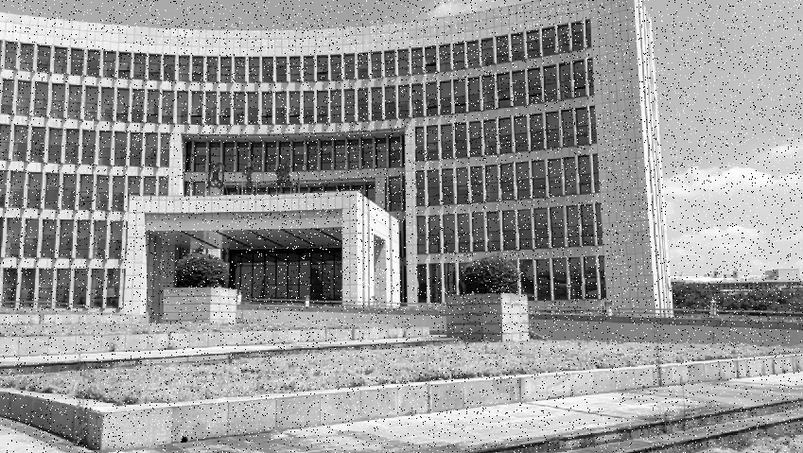
\includegraphics[width=\linewidth]{salt.png}
		\caption{椒盐噪声}
		\label{fig:椒盐噪声}
	\end{subfigure}
	\quad
	\begin{subfigure}[htpb]{.45\linewidth}
		\centering
		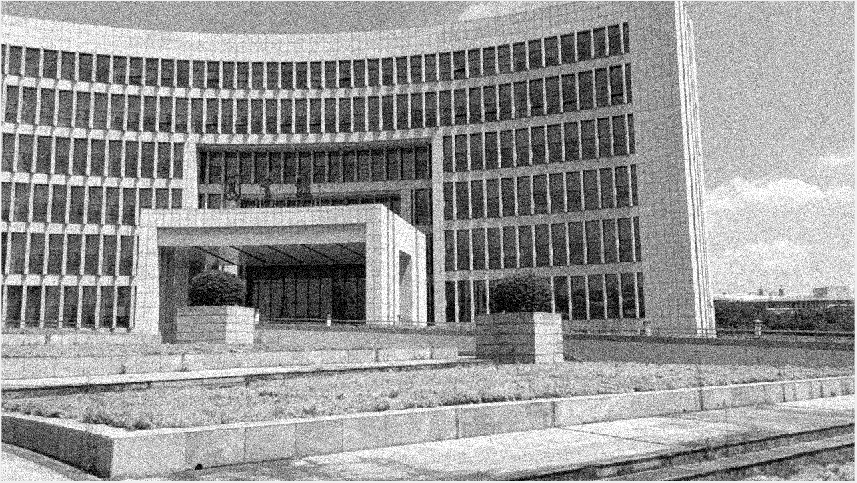
\includegraphics[width=\linewidth]{Gauss.png}
		\caption{高斯噪声}
		\label{fig:高斯噪声}
	\end{subfigure}
	\quad
	\begin{subfigure}[htpb]{.45\linewidth}
		\centering
		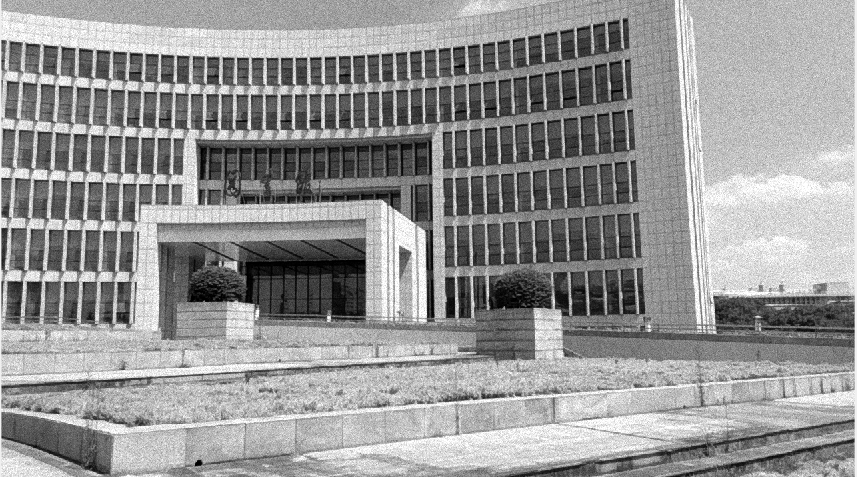
\includegraphics[width=\linewidth]{Possion.png}
		\caption{泊松噪声}
		\label{fig:泊松噪声}
	\end{subfigure}
	\quad
	\begin{subfigure}[htpb]{.45\linewidth}
		\centering
		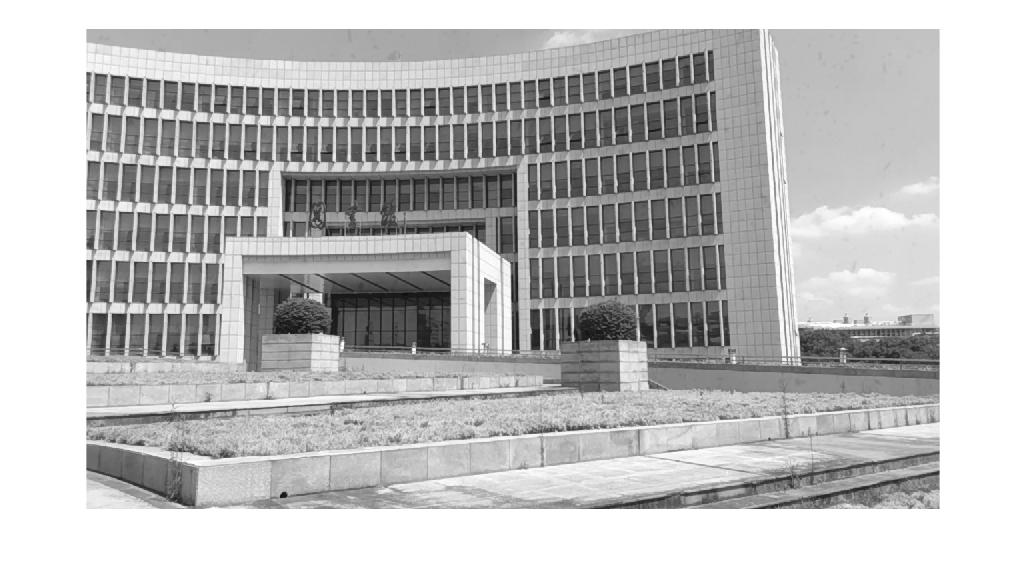
\includegraphics[width=\linewidth]{fixed.png}
		\caption{固定噪声}
		\label{fig:固定噪声}
	\end{subfigure}
	\quad
	\begin{subfigure}[htpb]{.45\linewidth}
		\centering
		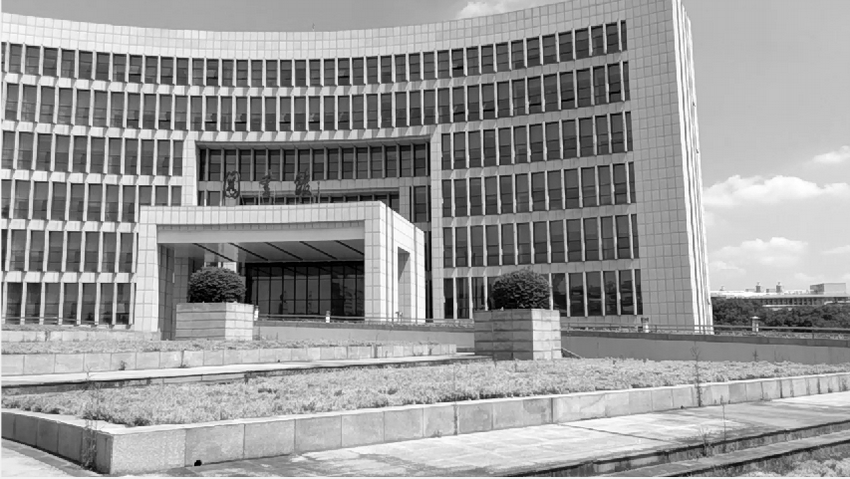
\includegraphics[width=\linewidth]{origin.png}
		\caption{原始图像}
		\label{fig:原始图像}
	\end{subfigure}
	\quad
	\caption{图像}
	\label{fig:图像}
\end{figure}

若对$ 720\times 1280 $个像素进行机器学习,则计算量过大,仿真时间过长。考虑到研究性质,可直接对视频中单一像素点位置进行处理。

硬件运行流程如图\ref{fig:硬件流程图}。

\begin{figure}[htpb]
	\centering
	\includegraphics[width=0.8\linewidth]{dia.pdf}
	\caption{硬件流程图}
	\label{fig:硬件流程图}
\end{figure}

\subsubsection{椒盐噪声}%
\label{ssub:椒盐噪声}

在学习速度为0.05,动量因子为0.001,原始图像在加入密度参数为0.05的椒盐噪声的情况下,明显图像的误差偏移减小,同时最后由于噪声过大偏差脱离的原精度水准的帧步数增大,对盲元和误差修订的次数减小。可见相应的结构能够明显的在椒盐噪声的情况下,对其进行修订与抑制。

\begin{figure}[htpb]
	\centering
	\begin{subfigure}[htpb]{.45\linewidth}
		\centering
		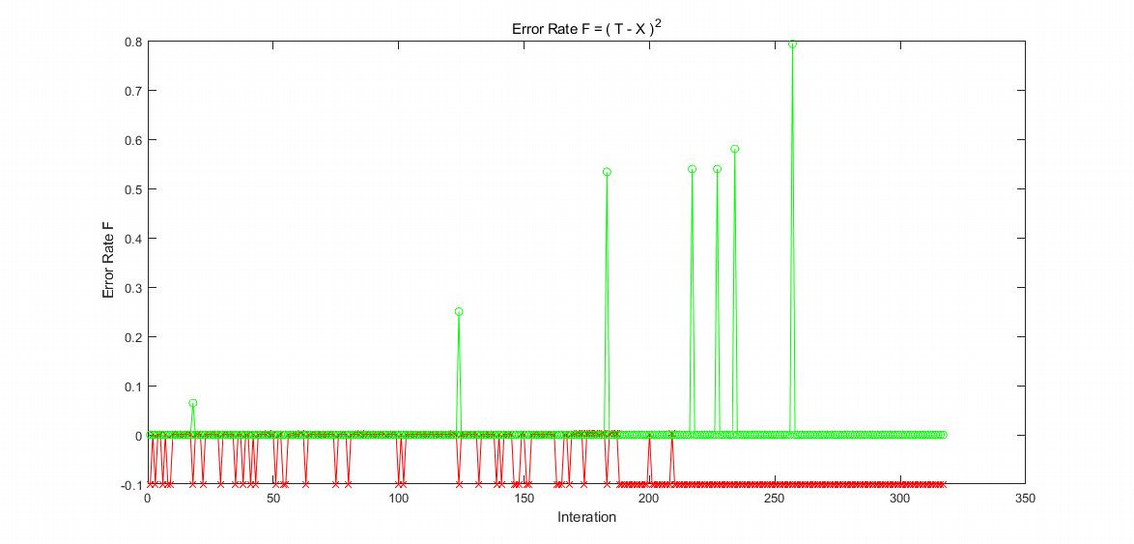
\includegraphics[width=\linewidth]{salt-5.png}
		\caption{椒盐噪声经过原始BP算法处理后的结果}
		\label{fig:椒盐噪声经过原始BP算法处理后的结果}
	\end{subfigure}
	\quad
	\begin{subfigure}[htpb]{.45\linewidth}
		\centering
		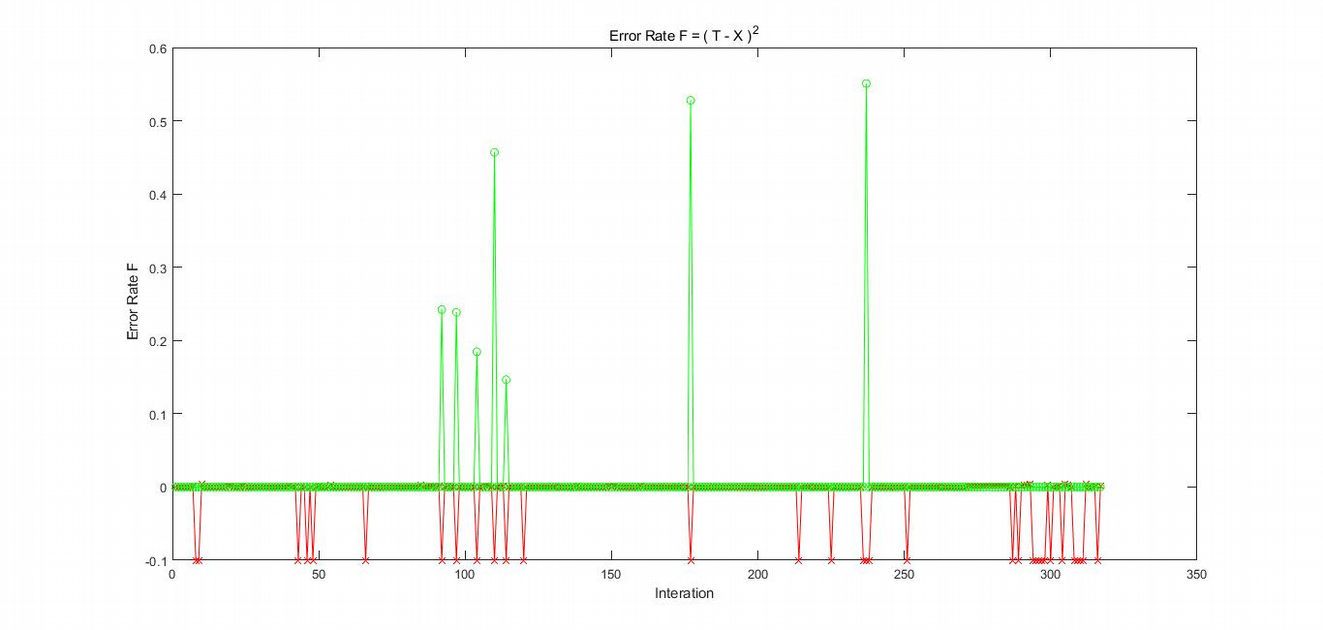
\includegraphics[width=\linewidth]{salt-9.png}
		\caption{椒盐噪声经过9像素BP算法处理后的结果}
		\label{fig:椒盐噪声经过9像素BP算法处理后的结果}
	\end{subfigure}
	\quad
	\begin{subfigure}[htpb]{.45\linewidth}
		\centering
		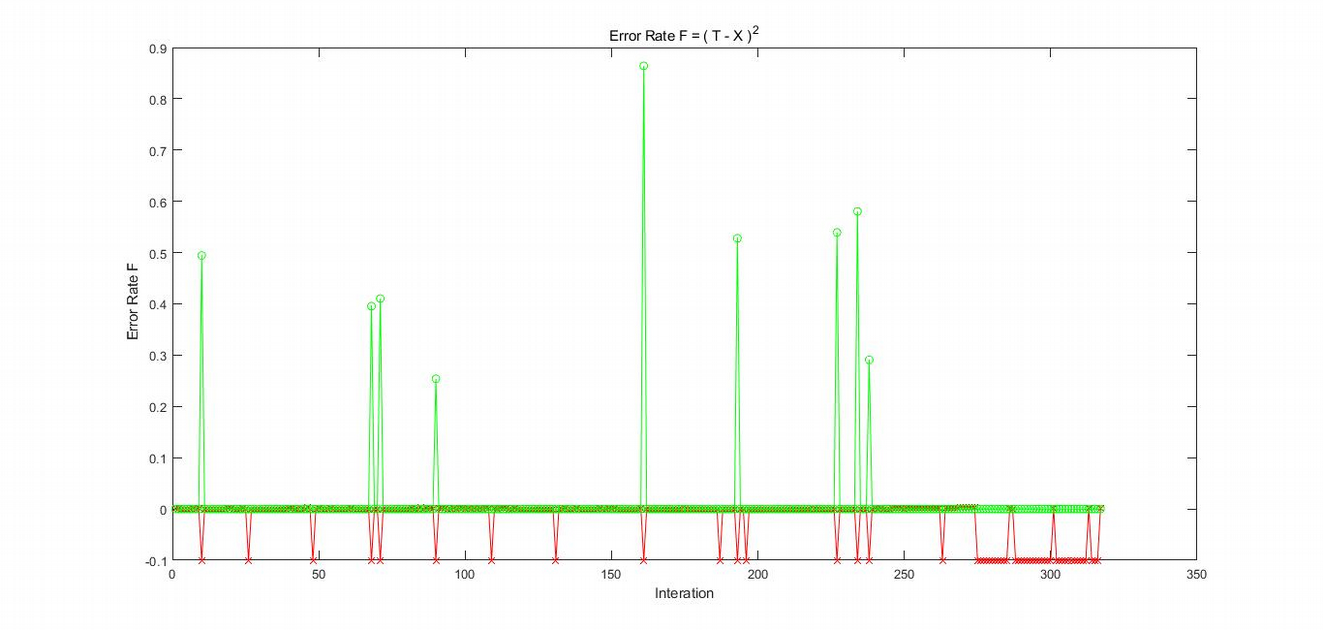
\includegraphics[width=\linewidth]{salt-13.png}
		\caption{椒盐噪声经过13像素BP算法处理后的结果}
		\label{fig:椒盐噪声经过13像素BP算法处理后的结果}
	\end{subfigure}
	\caption{椒盐噪声经过BP算法处理后的结果}
	\label{fig:椒盐噪声经过BP算法处理后的结果}
\end{figure}

\subsubsection{高斯噪声}%
\label{ssub:高斯噪声}

原始图像在加入均值为0,方差为0.01的高斯噪声的情况下,明显在高斯噪声下,三种方式的像素还原效果较佳,其中改进BP算法的帧频步长更长,且两种改进方式的效果基本一致。

\begin{figure}[htpb]
	\centering
	\begin{subfigure}[htpb]{.45\linewidth}
		\centering
		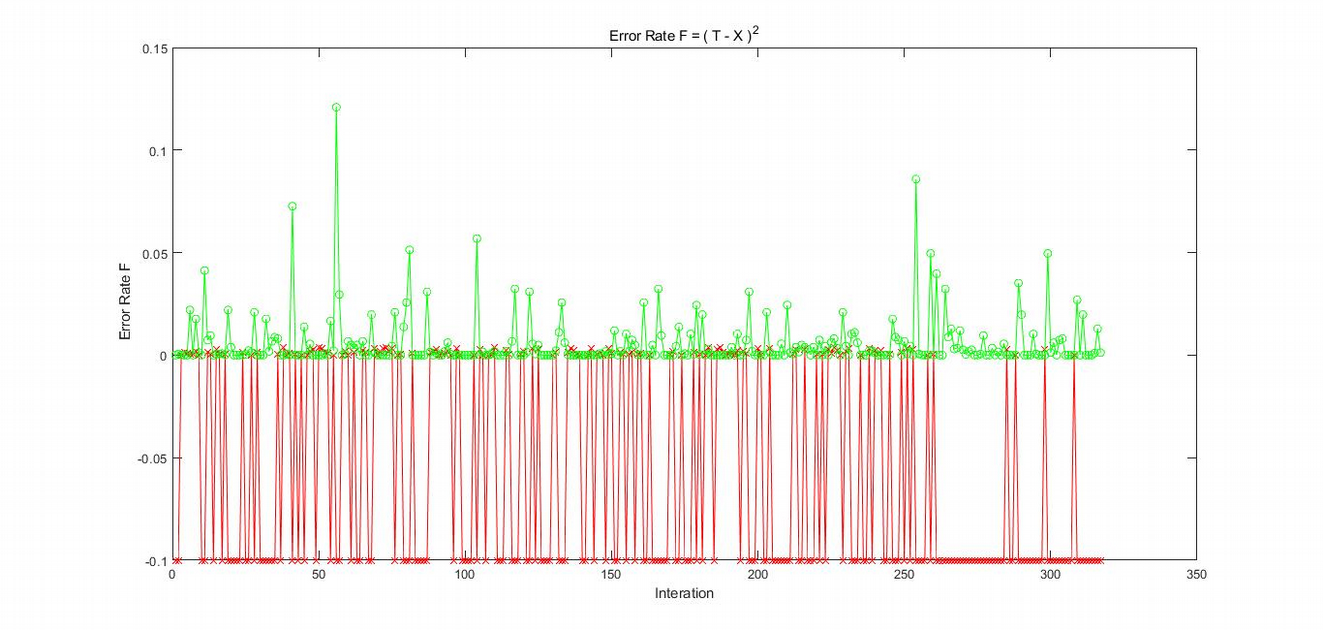
\includegraphics[width=\linewidth]{Gauss-5.png}
		\caption{高斯噪声经过原始BP算法处理后的结果}
		\label{fig:高斯噪声经过原始BP算法处理后的结果}
	\end{subfigure}
	\quad
	\begin{subfigure}[htpb]{.45\linewidth}
		\centering
		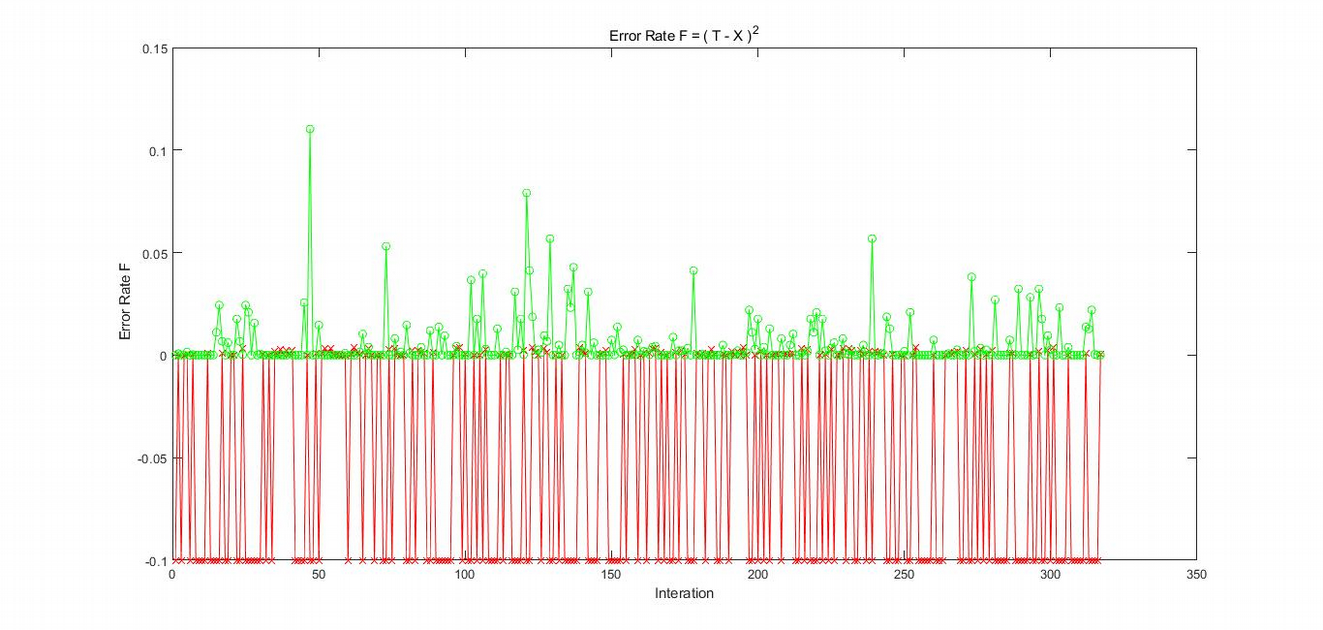
\includegraphics[width=\linewidth]{Gauss-9.png}
		\caption{高斯噪声经过9像素BP算法处理后的结果}
		\label{fig:高斯噪声经过9像素BP算法处理后的结果}
	\end{subfigure}
	\quad
	\begin{subfigure}[htpb]{.45\linewidth}
		\centering
		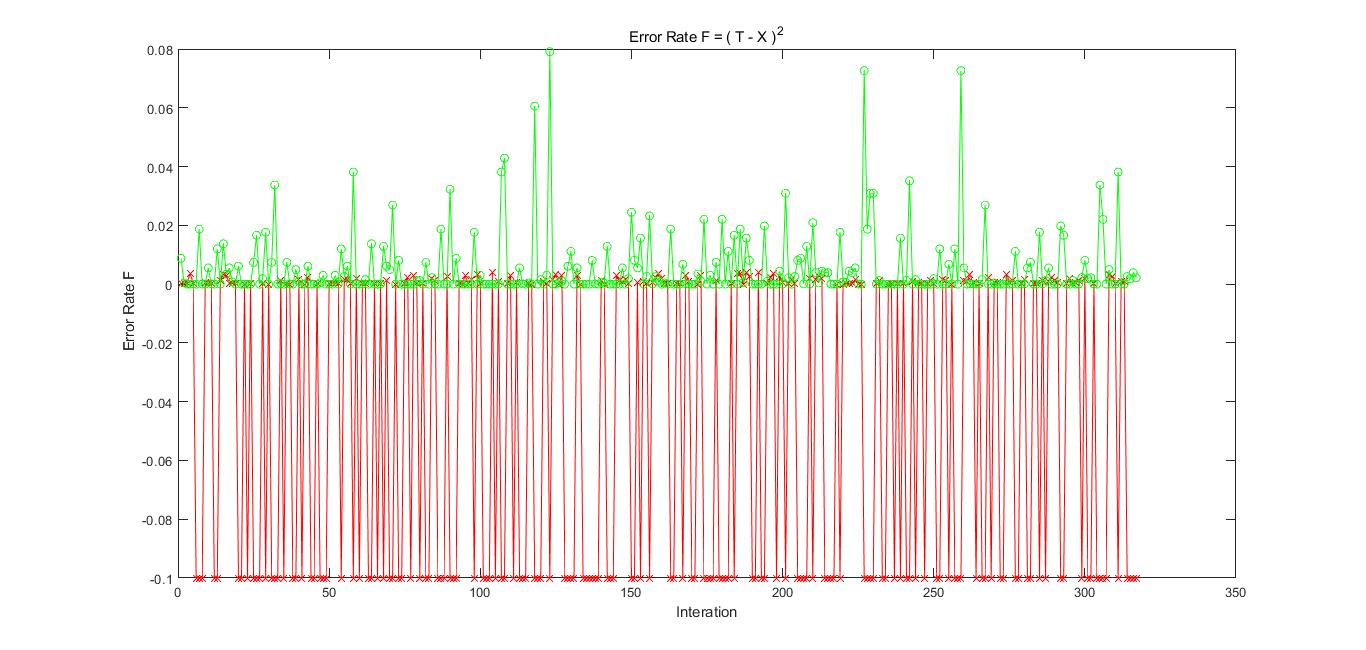
\includegraphics[width=\linewidth]{Gauss-13.png}
		\caption{高斯噪声经过13像素BP算法处理后的结果}
		\label{fig:高斯噪声经过13像素BP算法处理后的结果}
	\end{subfigure}
	\caption{高斯噪声经过BP算法处理后的结果}
	\label{fig:高斯噪声经过BP算法处理后的结果}
\end{figure}

\subsubsection{泊松噪声}%
\label{ssub:泊松噪声}

原始图像在加入泊松噪声的情况下,在泊松噪声下,三种方式的BP算法成效均可。但是就效果而言,仍然是中值滤波方式的BP算法能够更好的还原图像像素的原始数值。

\begin{figure}[htpb]
	\centering
	\begin{subfigure}[htpb]{.45\linewidth}
		\centering
		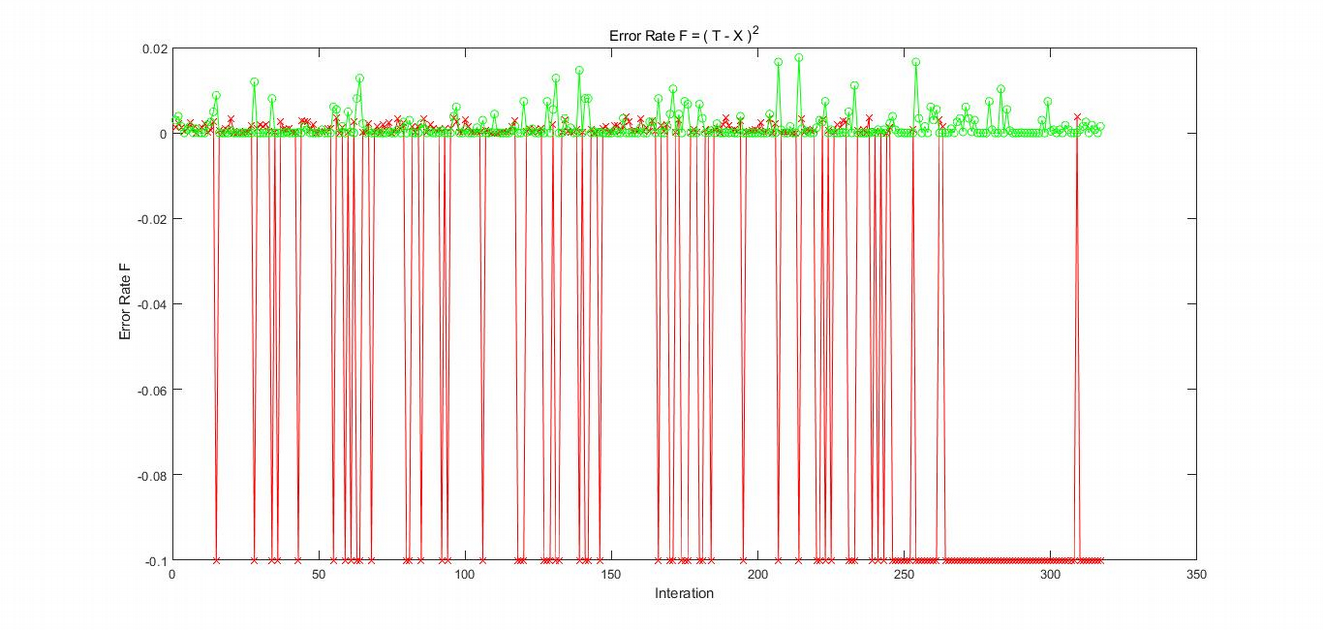
\includegraphics[width=\linewidth]{Possion-5.png}
		\caption{泊松噪声经过原始BP算法处理后的结果}
		\label{fig:泊松噪声经过原始BP算法处理后的结果}
	\end{subfigure}
	\quad
	\begin{subfigure}[htpb]{.45\linewidth}
		\centering
		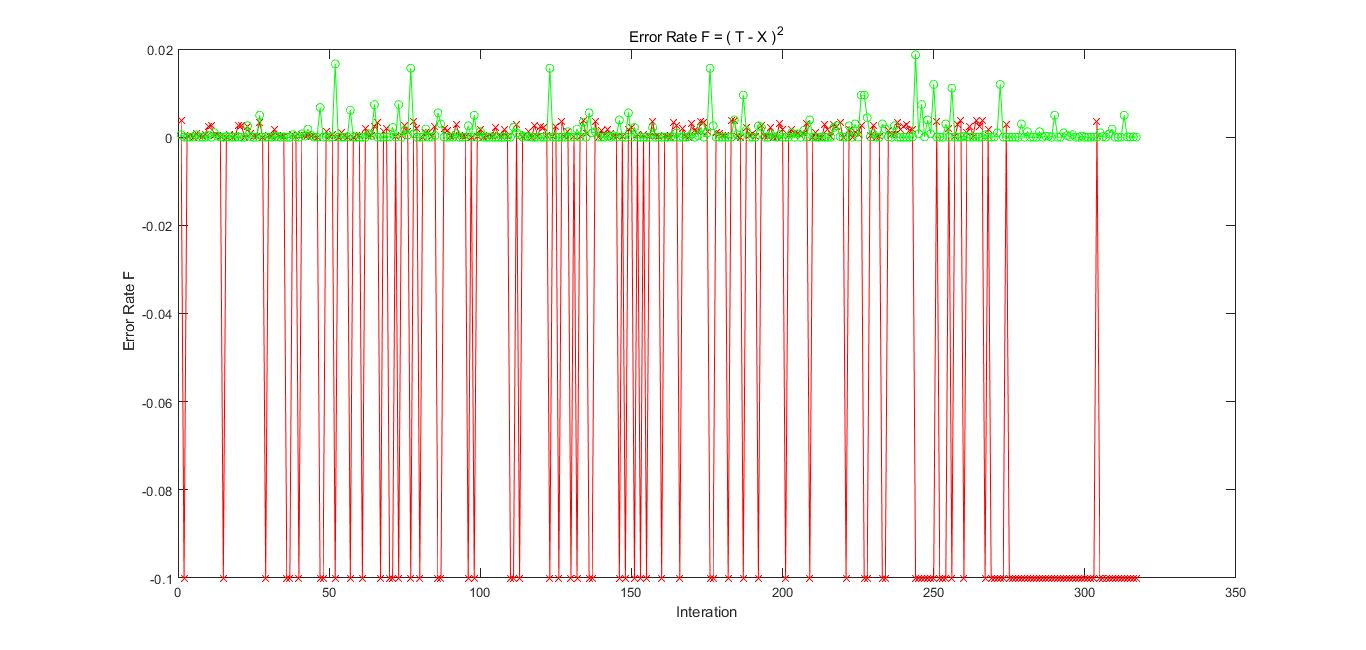
\includegraphics[width=\linewidth]{Possion-9.png}
		\caption{泊松噪声经过9像素BP算法处理后的结果}
		\label{fig:泊松噪声经过9像素BP算法处理后的结果}
	\end{subfigure}
	\quad
	\begin{subfigure}[htpb]{.45\linewidth}
		\centering
		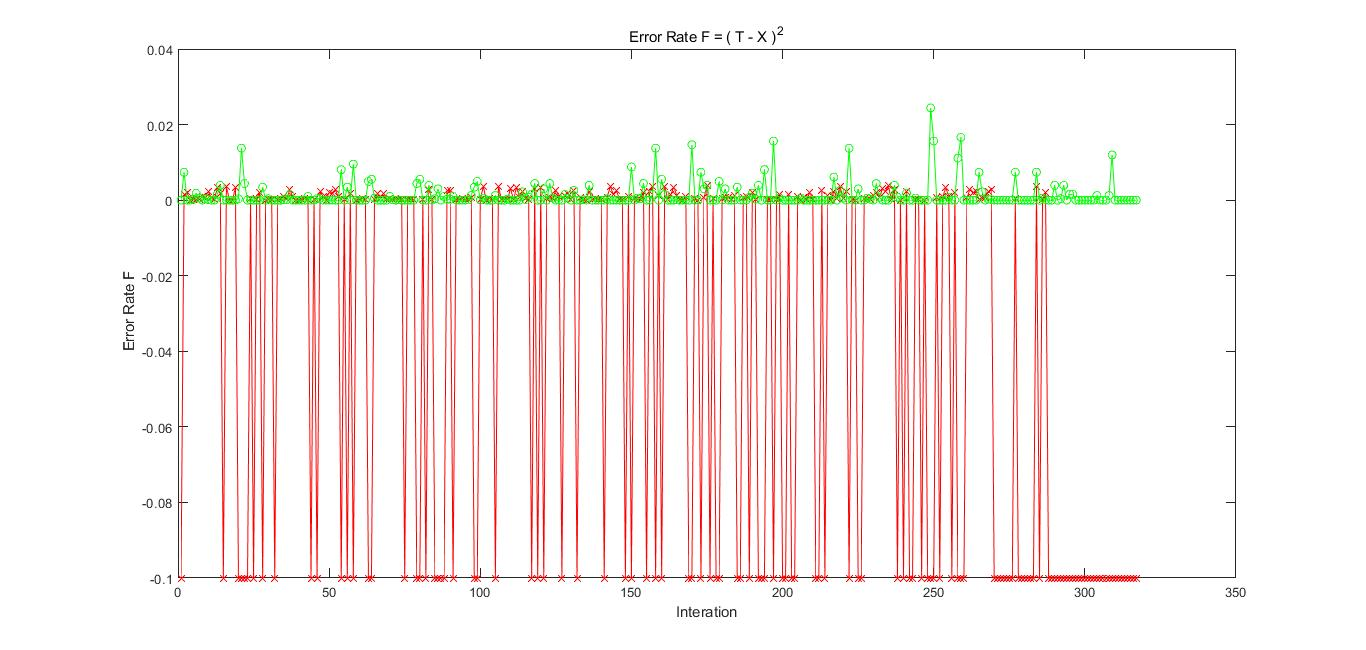
\includegraphics[width=\linewidth]{Possion-13.png}
		\caption{泊松噪声经过13像素BP算法处理后的结果}
		\label{fig:泊松噪声经过13像素BP算法处理后的结果}
	\end{subfigure}
	\caption{泊松噪声经过BP算法处理后的结果}
	\label{fig:泊松噪声经过BP算法处理后的结果}
\end{figure}

\subsubsection{固定噪声}%
\label{ssub:固定噪声}

原始图像在加入固定噪声的情况下,明显改进的BP算法形式,相比于一般的BP算法形式具有更加低的Error Rate。但是在帧数增加后仍然存在Error rate 上升的情况。

\begin{figure}[htpb]
	\centering
	\begin{subfigure}[htpb]{.45\linewidth}
		\centering
		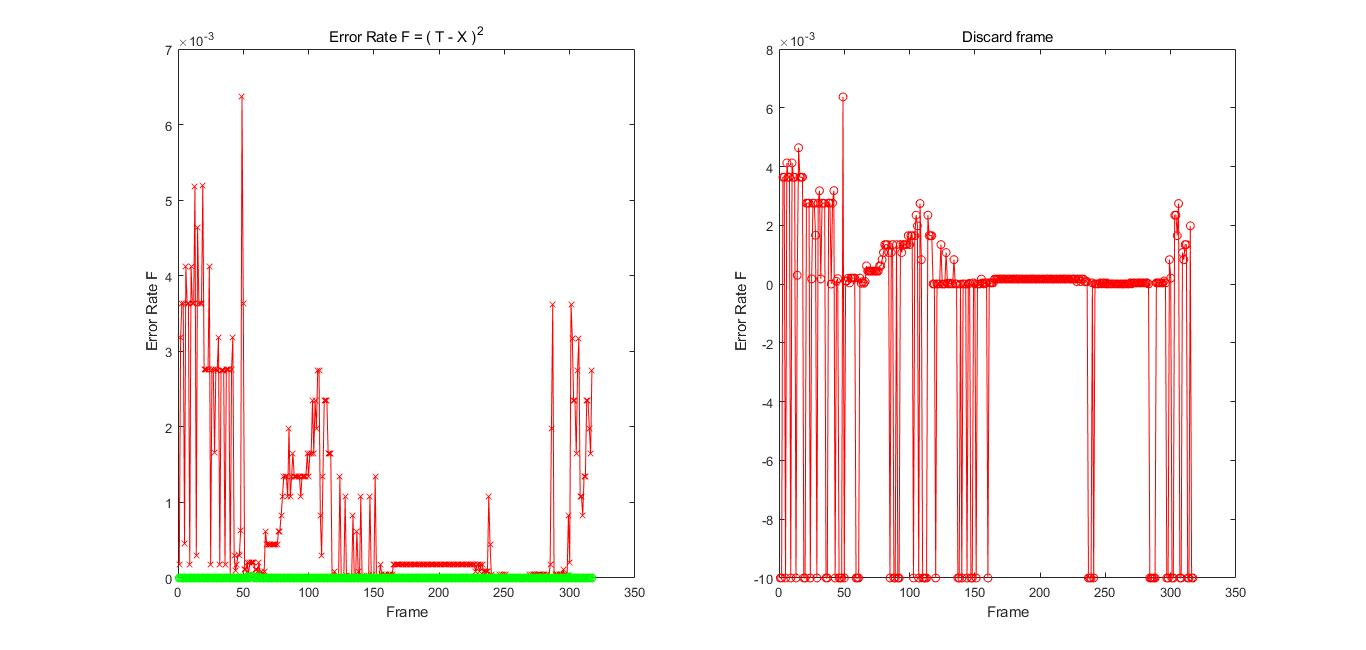
\includegraphics[width=\linewidth]{fixed-5.png}
		\caption{固定噪声经过原始BP算法处理后的结果}
		\label{fig:固定噪声经过原始BP算法处理后的结果}
	\end{subfigure}
	\quad
	\begin{subfigure}[htpb]{.45\linewidth}
		\centering
		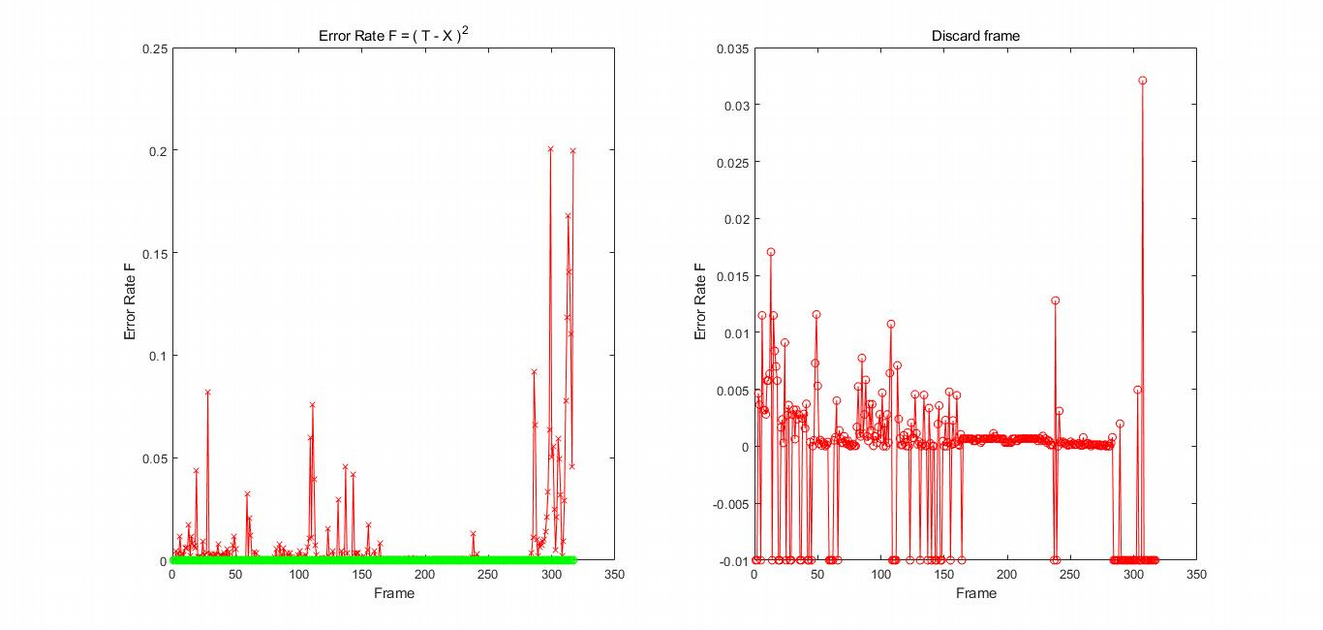
\includegraphics[width=\linewidth]{fixed-9.png}
		\caption{固定噪声经过9像素BP算法处理后的结果}
		\label{fig:固定噪声经过9像素BP算法处理后的结果}
	\end{subfigure}
	\quad
	\begin{subfigure}[htpb]{.45\linewidth}
		\centering
		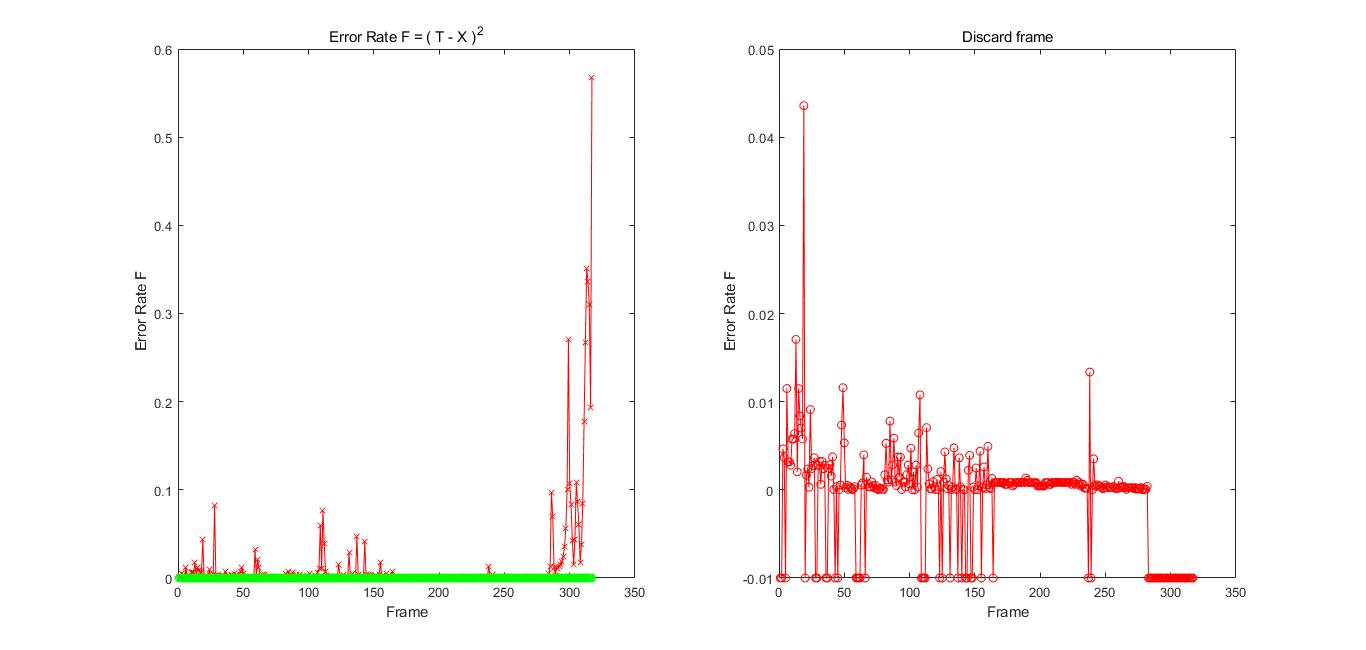
\includegraphics[width=\linewidth]{fixed-13.png}
		\caption{固定噪声经过13像素BP算法处理后的结果}
		\label{fig:固定噪声经过13像素BP算法处理后的结果}
	\end{subfigure}
	\caption{固定噪声经过BP算法处理后的结果}
	\label{fig:固定噪声经过BP算法处理后的结果}
\end{figure}

\subsection{创新之处}%
\label{sub:创新之处}

在改进BP神经网络的算法下,对单个像素点的情况进行了像点数值恢复仿真,并且取得了较好的效果。在椒盐噪声、高斯噪声、泊松噪声和固定图像噪声四种噪声污染图片的情况下,验证了中值滤波作为$ T $函数对于BP神经网络算法的优越性。

\newpage

\section{科学意义及前景}%
\label{sec:科学意义及前景}

\subsection{科学意义}%
\label{sub:科学意义}

在改进BP神经网络的算法下,对单个像素点的情况进行了像点数值恢复仿真,并且取得了较好的效果。在椒盐噪声,高斯噪声,泊松噪声和固定图像噪声四种噪声污染图片的情况下,验证了中值滤波作为T函数对于BP神经网络算法的优越性。

但目前仍然存在着一些问题。在仿真实验中,学习速度与动量因子是固定值。但是在实际的情况下,最优的解决方式需要根据图像的不同特征对学习速度与动量因子进行修订,目前还未找到合理的方法如何动态的修订这两个参数。

\subsection{前景}%
\label{sub:前景}

红外辐射的探测在军事和民用上有着广泛的运用需求。在第二次世界大战后,现代的红外传感器技术进入了初期阶段,在20世纪50到60年代,使用的单元致冷铅盐探测器制作的红外传感器首次进入用于防空导弹的寻的,从此开始了红外在军事上的应用。目前,红外技术已经从军事应用转向民用,在国民经济各个领域发挥着重要的作用而随着红外焦平面探测器的出现,红外成像系统进入了一个新的时期。

红外探测技术的领先将使得我国在军事和民用领域占有巨大优势,这是由于红外探测的特点决定的:首先是对环境的适应能力比可见光要好,特别是在黑夜和恶劣天气下;其次是隐蔽性能好,它被动接受目标的信号,比雷达和激光等探测器安全;还有,它利用目标和背景之间的温差所形成的热辐射特性进行探测,其识别目标的能力非常强。

\newpage

\section{研究目标的达成度分析}%
\label{sec:研究目标的达成度分析}

目前仍然存在着一些问题。在仿真实验中,学习速度与动量因子是固定值。但是在实际的情况下,最优的解决方式需要根据图像的不同特征对学习速度与动量因子进行修订,目前还未找到合理的方法如何动态的修订这两个参数。

同时随着BP算法的运行,会发现最后整体像素都会产生一定的灰度飘逸。虽然对于红外图像高背景本底低分辨率的特性而言,相应的灰度层级变化影响并不是很大,但是仍然需要进行整体的灰度补偿。

\end{document}

